\section{Tutorial}



\begin{frame}
  \heading{Let's step into \odeint}
  \tableofcontents[currentsection] 
\end{frame}


\begin{frame}[fragile]

\heading{Example -- Pendulum}

\vspace{2ex}

\begin{columns}[T]
  \begin{column}{0.35\textwidth}
    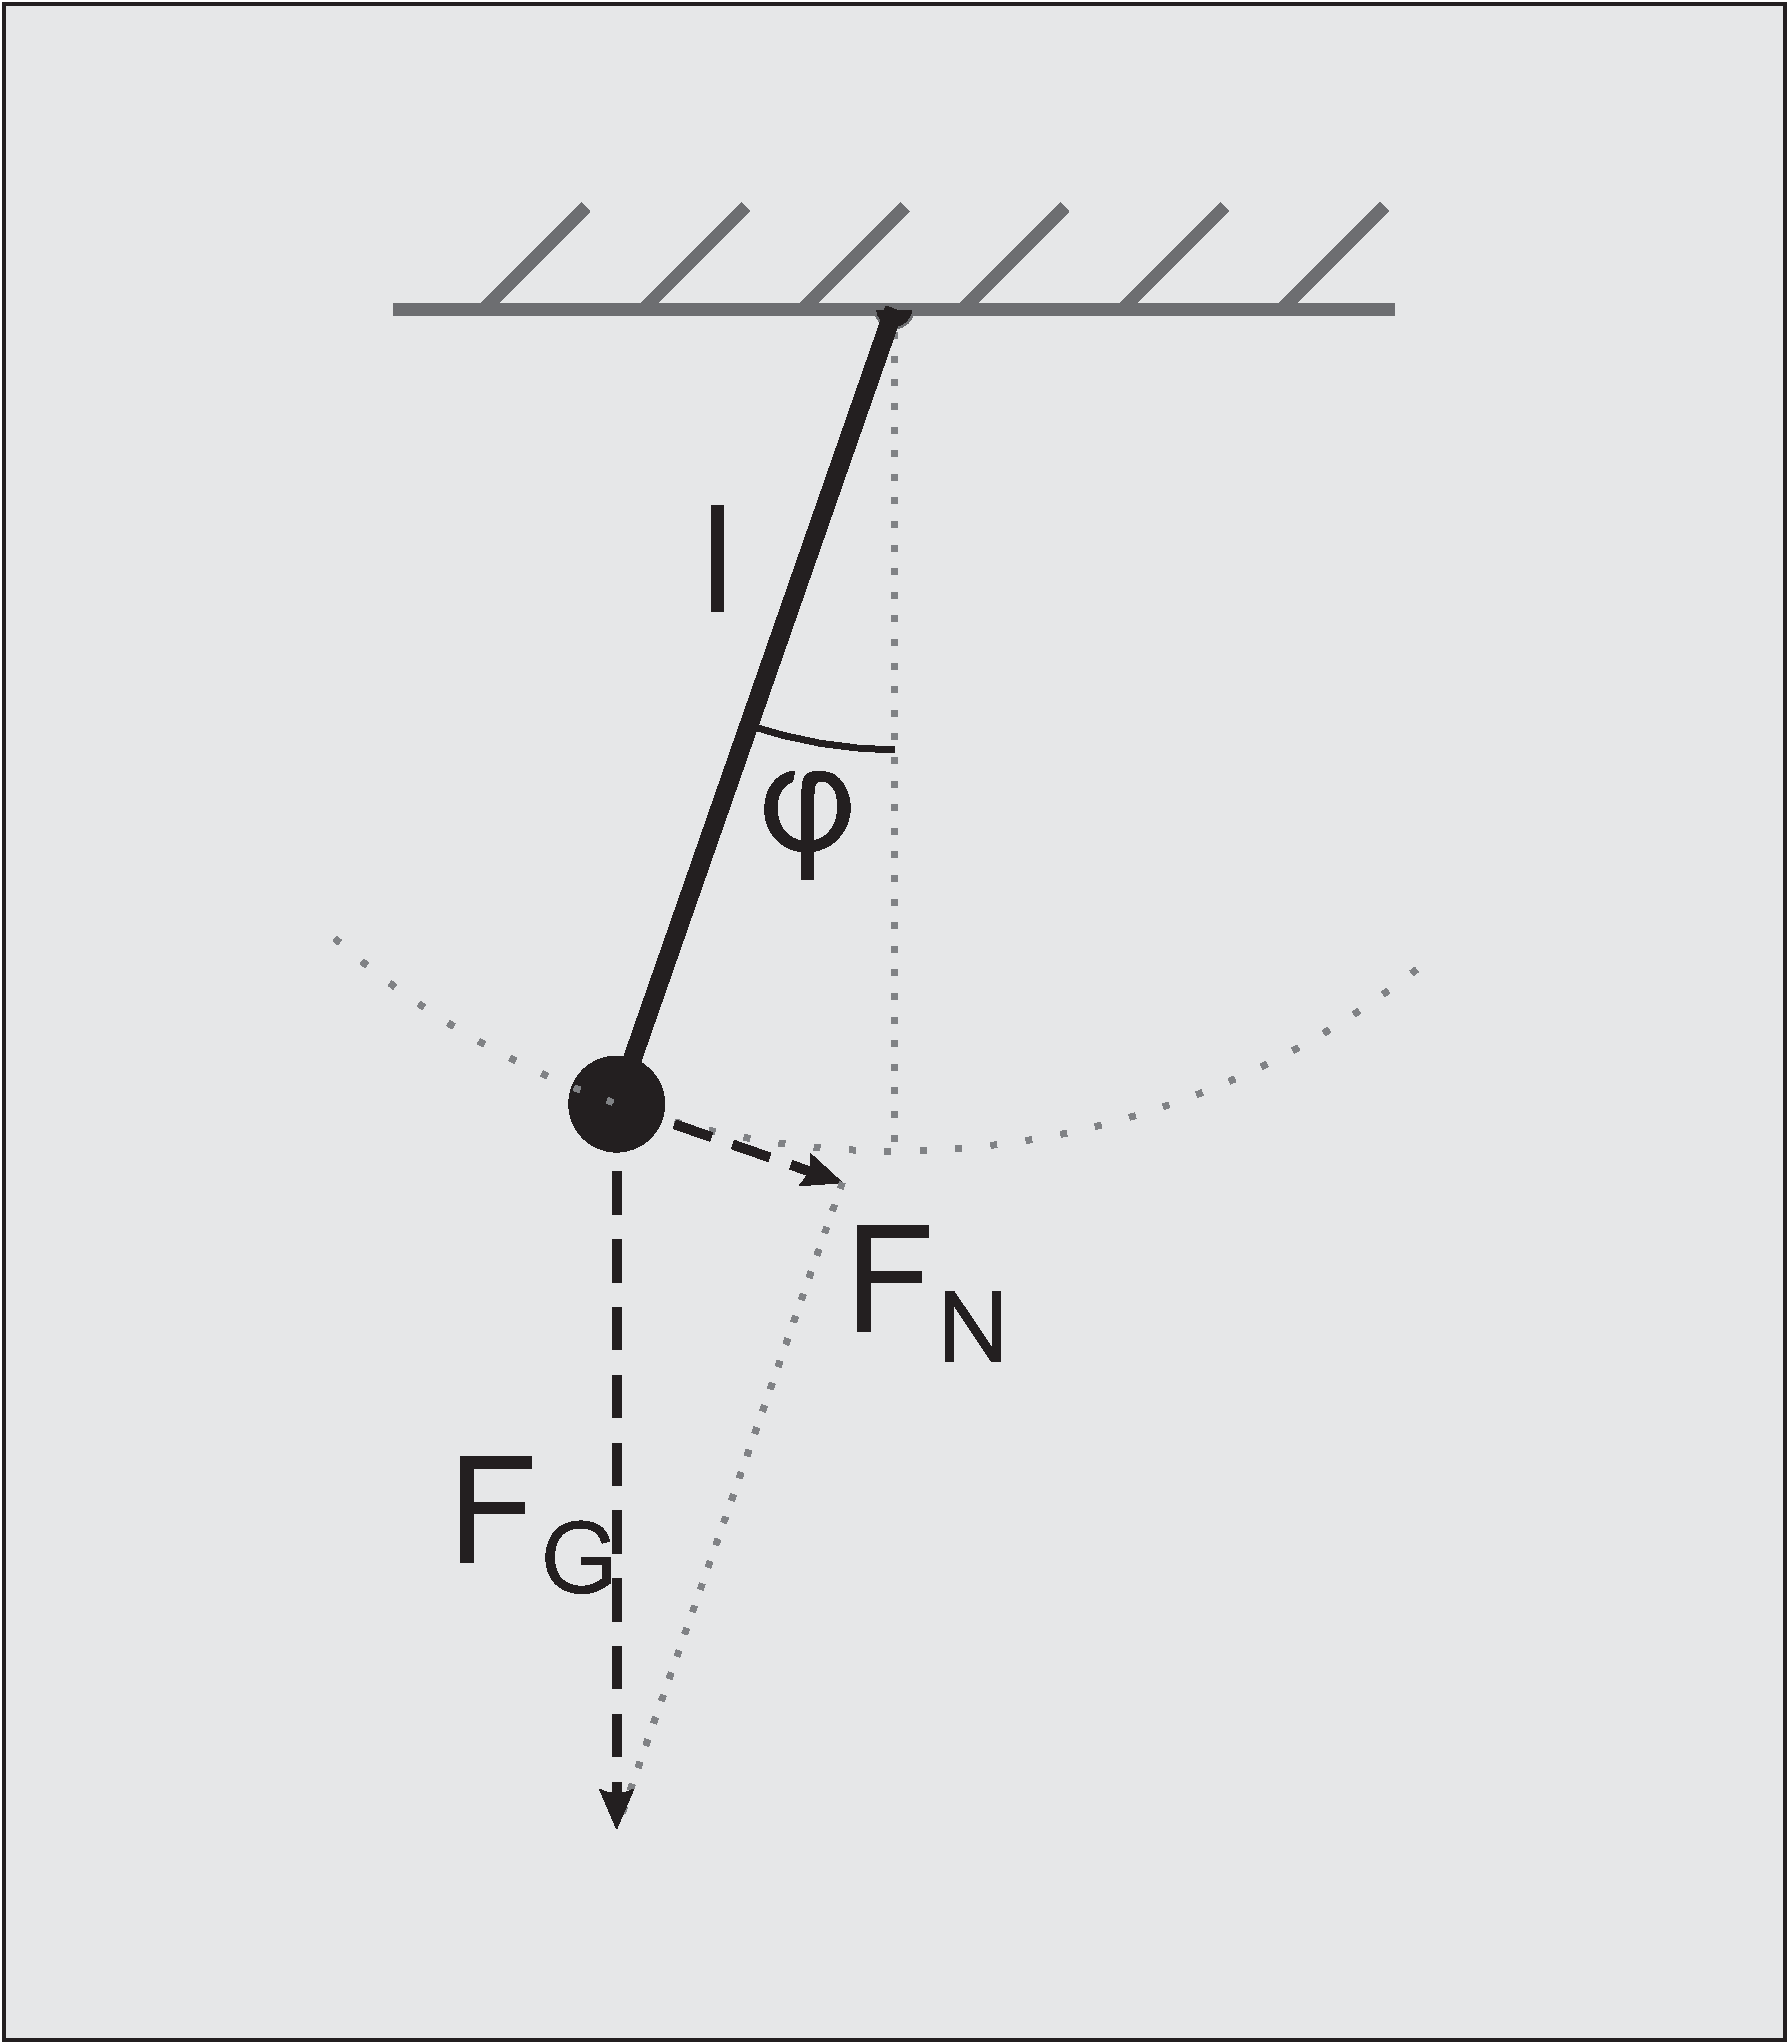
\includegraphics[draft=false,width=1.0\textwidth]{pendulum.pdf}

   \vspace{4ex}
  \end{column}

  \begin{column}{0.65\textwidth}
 \only<1>{
 Newtons law: $m a = F$

 \vspace{2ex}

 Acceleration:  $a = l \ddot{\varphi} = \frac{\de^2 \varphi}{\de t^2} $

 \vspace{2ex}

 Force: $F=F_N = - m g \sin \varphi$

 \vspace{4ex}

 $\Longrightarrow$ {\bf ODE for $\varphi$}

 $$\ddot{\varphi} = - g / l \sin \varphi = -\omega_0^2 \sin \varphi$$
 }

 \only<2>
 {

 $$\ddot{\varphi} = - \omega_0^2 \sin \varphi $$

 Small angle: $\sin \varphi \approx \varphi$

 \vspace{2ex}

 Harmonic oscillator $\ddot{\varphi} = - \omega_0^2 \varphi$

 \vspace{2ex}

 Analytic solution: $\varphi = A \cos \omega_0 t + B \sin \omega_0 t$

 \vspace{2ex}

 Determine $A$ and $B$ from initial condition\rem{:

 \centerline{$\varphi(t=0) = \varphi_0 \,\, \text{,} \quad \dot{\varphi}(t=0) = \dot{\varphi}_0$}

 \centerline{$B=\varphi_0 \,\, \text{,} \quad A=\dot{\varphi}_0 / \omega$}}

 }

 \only<3>{

 Full equation: $\ddot{\varphi} = -\omega_0^2 \sin \varphi $

 \vspace{2ex}

 Pendulum with friction and external driving:

 $$\ddot{\varphi} = -\omega_0^2 \sin \varphi - \mu \dot{\varphi} + \varepsilon \sin \omega_E t $$

 \vspace{2ex}

 No analytic solution is known

 \vspace{2ex}

 $\Longrightarrow$ {\bf Solve this equation numerically.}

 }

 \only<4>{

 $$\ddot{\varphi} = -\omega_0^2 \sin \varphi - \mu \dot{\varphi} + \varepsilon \sin \omega_E t $$

 \vspace{2ex}

 Create a first order ODE

 \vspace{1ex}

 \centerline{$x_1 = \varphi \,\, \text{,} \quad x_2 = \dot{\varphi}$}

 \vspace{-3ex}
 \begin{align*}
   \dot{x_1} &= x_2 \\
   \dot{x_2} &= - \omega_0  \sin x_1 - \mu x_2 + \varepsilon \sin \omega_E t  
 \end{align*}


 $x_1$ and $x_2$ are the state space variables

 }
   
  \end{column}
\end{columns}

 

\end{frame}







\begin{frame}[fragile]

\centerline{ \Large Let's solve the pendulum example numerically}

\vspace{2ex}
\begin{lstlisting}
#include <boost/numeric/odeint.hpp>

namespace odeint = boost::numeric::odeint;
\end{lstlisting}

\vspace{2ex}

\centerline{$\dot{x_1} = x_2 \,\,\text{,} \quad \dot{x_2} = - \omega_0 \sin x_1 - \mu x_2 + \varepsilon \sin \omega_E t$}

\vspace{2ex}
\begin{lstlisting}
typedef std::array<double,2> state_type;
\end{lstlisting}

\end{frame}

\begin{frame}[fragile]

\centerline{ \Large Let's solve the pendulum example numerically}

\vspace{2ex}

$\dot{x_1} = x_2$, $\dot{x_2} = - \omega_0^2 \sin x_1 - \mu x_2 + \varepsilon \sin \omega_E t$ \hspace{6ex} $\omega_0^2 = 1$

\vspace{2ex}

\begin{lstlisting}
struct pendulum
{
  double m_mu, m_omega, m_eps;

  pendulum(double mu,double omega,double eps)
  : m_mu(mu),m_omega(omega),m_eps(eps) { }

  void operator()(const state_type &x,state_type &dxdt,double t) const
  {
    dxdt[0] = x[1];
    dxdt[1] = -sin(x[0]) - m_mu * x[1] +
        m_eps * sin(m_omega*t);
  }
};
\end{lstlisting}

\end{frame}

\begin{frame}[fragile]
 \centerline{ \Large Let's solve the pendulum example numerically}

\vspace{2ex}
$\varphi(0) = x_1(0) = 1 \,\, \text{,} \quad \dot{\varphi}(0) = x_2(0) = 0$
\vspace{2ex}

\begin{lstlisting}
odeint::runge_kutta4< state_type > rk4;
pendulum p( 0.1 , 1.05 , 1.5 );

state_type x = {{ 1.0 , 0.0 }};
double t = 0.0;

const double dt = 0.01;
rk4.do_step( p , x , t , dt );
t += dt;
\end{lstlisting}

\vspace{2ex}

\centerline{$x(0) \mapsto x(\Delta t)$}

\end{frame}

\begin{frame}[fragile]
 \centerline{ \Large Let's solve the pendulum example numerically}

\vspace{2ex}


\begin{lstlisting}
std::cout<<t<<" "<< x[0]<<" "<<x[1]<<"\n";
for( size_t i=0 ; i<10 ; ++i )
{
  rk4.do_step( p , x , t , dt );
  t += dt;
  std::cout<<t<<" "<< x[0]<<" "<<x[1]<<"\n";
}
\end{lstlisting}

\vspace{1ex}

\centerline{$x(0) \mapsto x(\Delta t) \mapsto x(2\Delta t) \mapsto x(3\Delta t) \mapsto \dots$}

\vspace{1ex}

\centerline{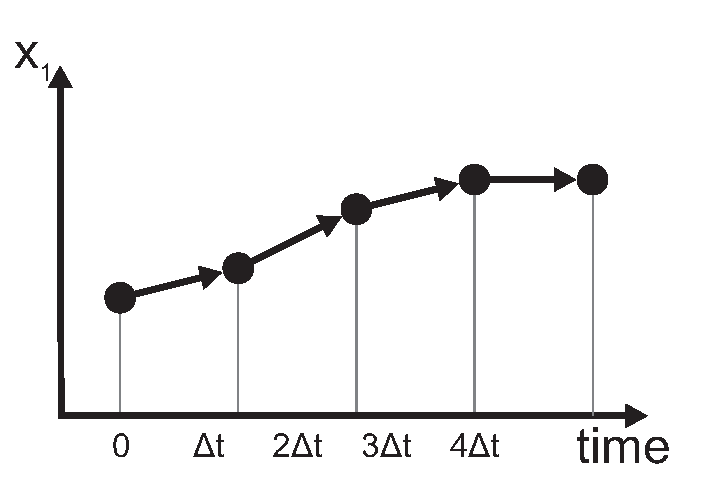
\includegraphics[draft=false,width=0.48\textwidth]{stepper_temporal_evolution.pdf}
\hspace{1ex}
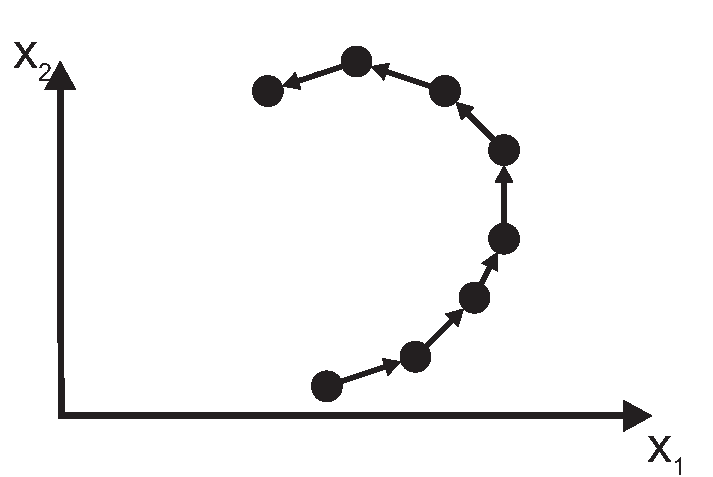
\includegraphics[draft=false,width=0.48\textwidth]{stepper_phase_space.pdf}}
\end{frame}


\rem{
\begin{frame}[fragile]
 \heading{Simulation}

 \vspace{1ex}

 \centerline{Oscillator: $\mu=0 \,\, \text{,} \quad \omega_E = 0 \,\, \text{,} \quad \varepsilon=0$}

 \vspace{1ex}

 \centerline{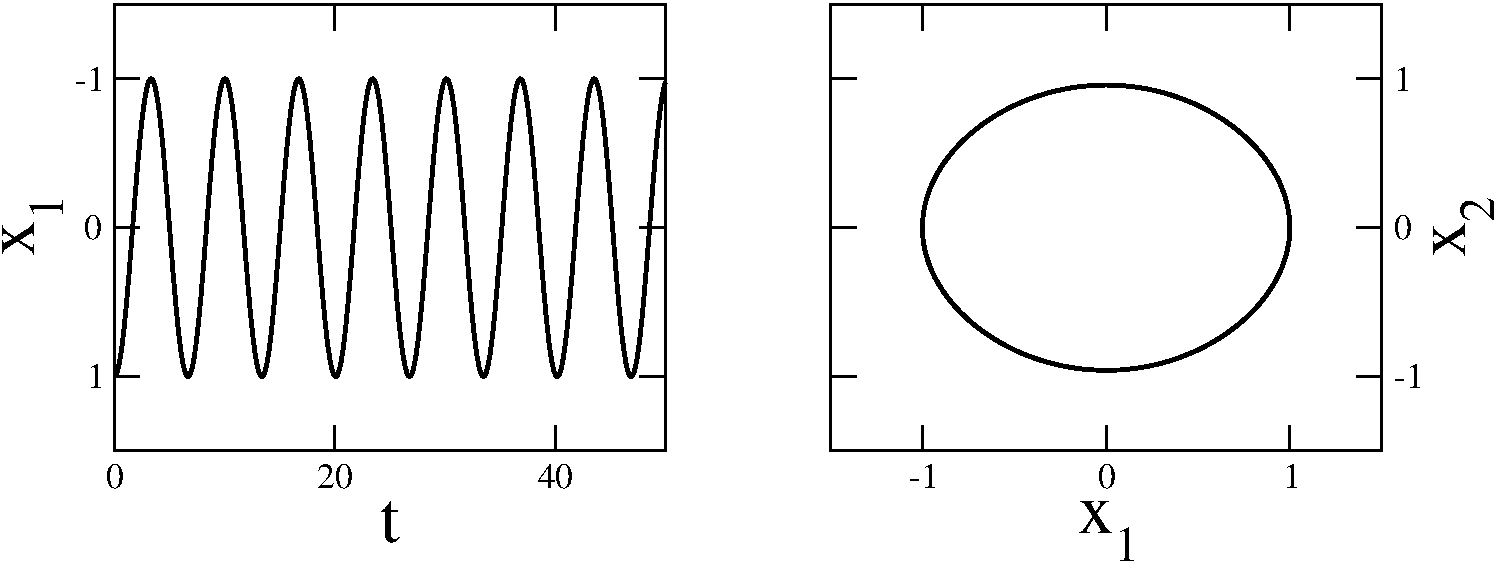
\includegraphics[draft=false,width=0.6\textwidth]{undamped.pdf}}

% \vspace{1ex}
 
\centerline{Damped oscillator: $\mu=0.1 \,\, \text{,} \quad \omega_E = 0 \,\, \text{,} \quad \varepsilon=0$}

 \vspace{1ex}

 \centerline{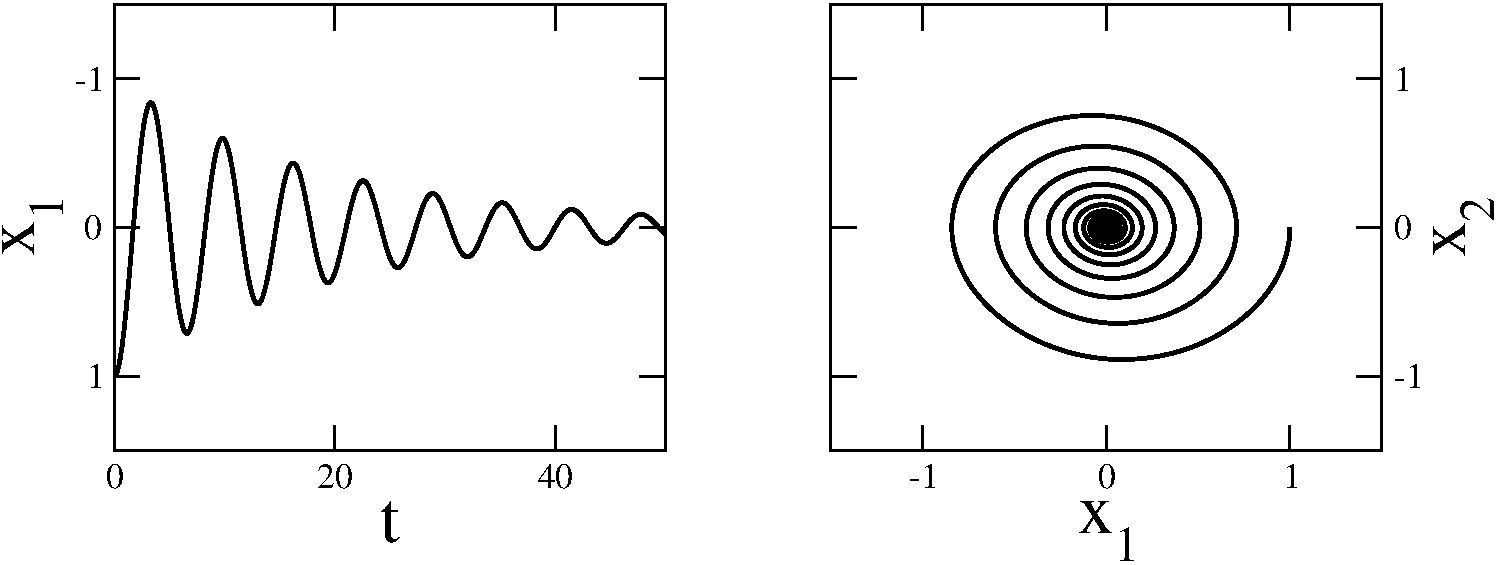
\includegraphics[draft=false,width=0.6\textwidth]{damped.pdf}}

% \vspace{1ex}

 \centerline{Damped, driven oscillator: $\mu=0.1 \,\, \text{,} \quad \omega_E = 1.05 \,\, \text{,} \quad \varepsilon=1.5$}

 \vspace{1ex}

 \centerline{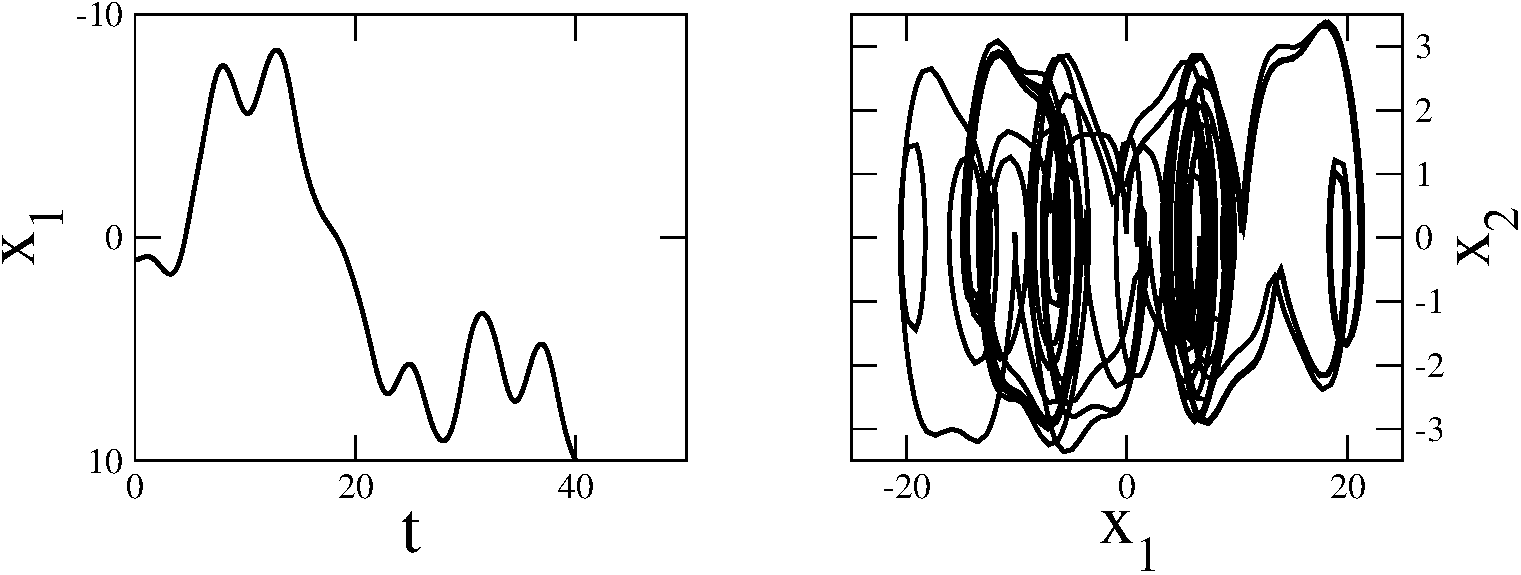
\includegraphics[draft=false,width=0.6\textwidth]{damped_driven.pdf}}


\end{frame}
}





\begin{frame}[fragile]
 \heading{Simulation}

 \vspace{2ex}

\begin{minipage}[t]{0.5\textwidth}
\vspace{0pt}
Oscillator

\vspace{1ex}
$\mu=0 \, \text{,} \,\, \omega_E = 0 \, \text{,} \,\, \varepsilon=0$

\vspace{7ex}
Damped oscillator:

\vspace{1ex}
$\mu=0.1  \, \text{,} \,\, \omega_E = 0  \, \text{,} \,\, \varepsilon=0$

\vspace{7ex}
Damped, driven oscillator:

\vspace{1ex}
$\mu=0.1  \, \text{,} \,\, \omega_E = 1.05  \, \text{,} \,\, \varepsilon=1.5$
\end{minipage}\pause
\begin{minipage}[t]{0.49\textwidth}
\vspace{0pt}
\centerline{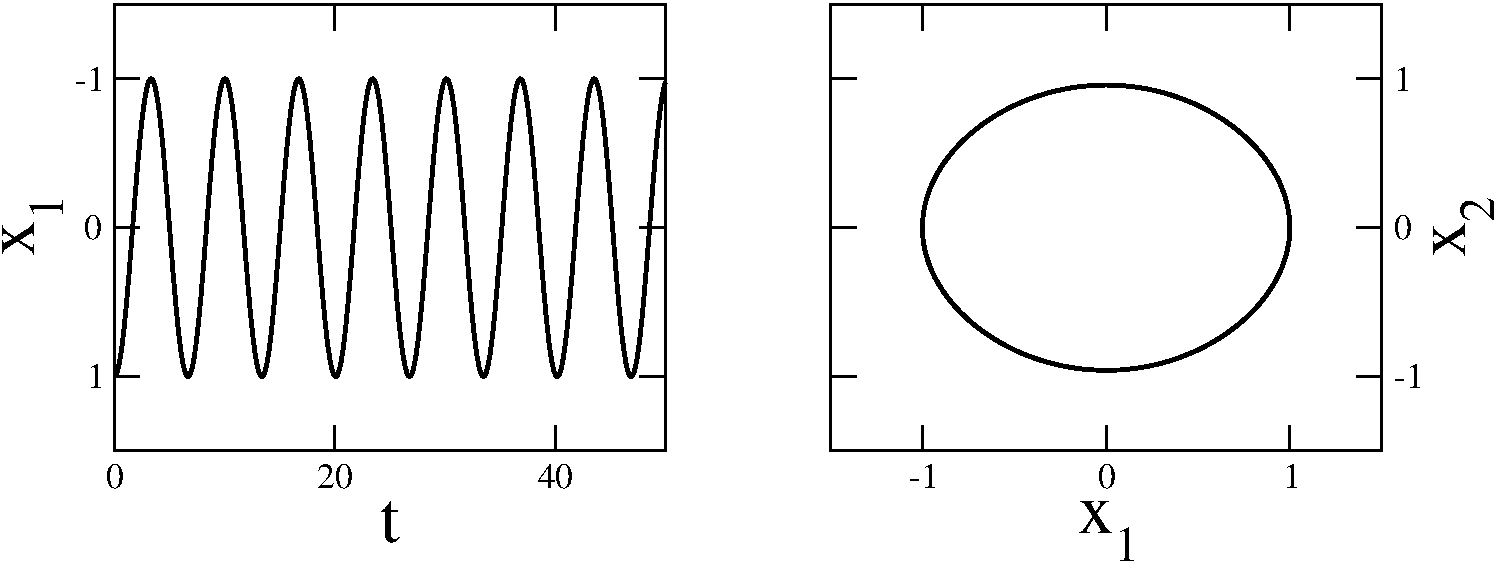
\includegraphics[draft=false,width=1.0\textwidth]{undamped.pdf}}

\vspace{2.5ex}
\centerline{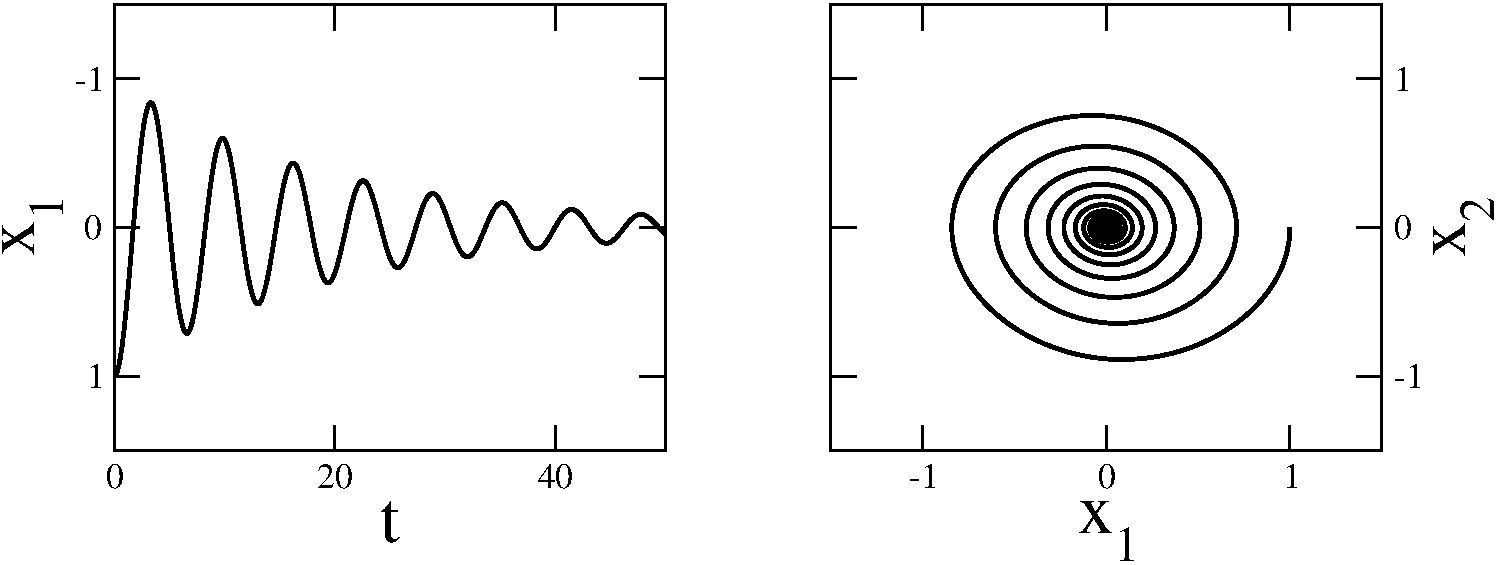
\includegraphics[draft=false,width=1.0\textwidth]{damped.pdf}}

\vspace{2.5ex}
\centerline{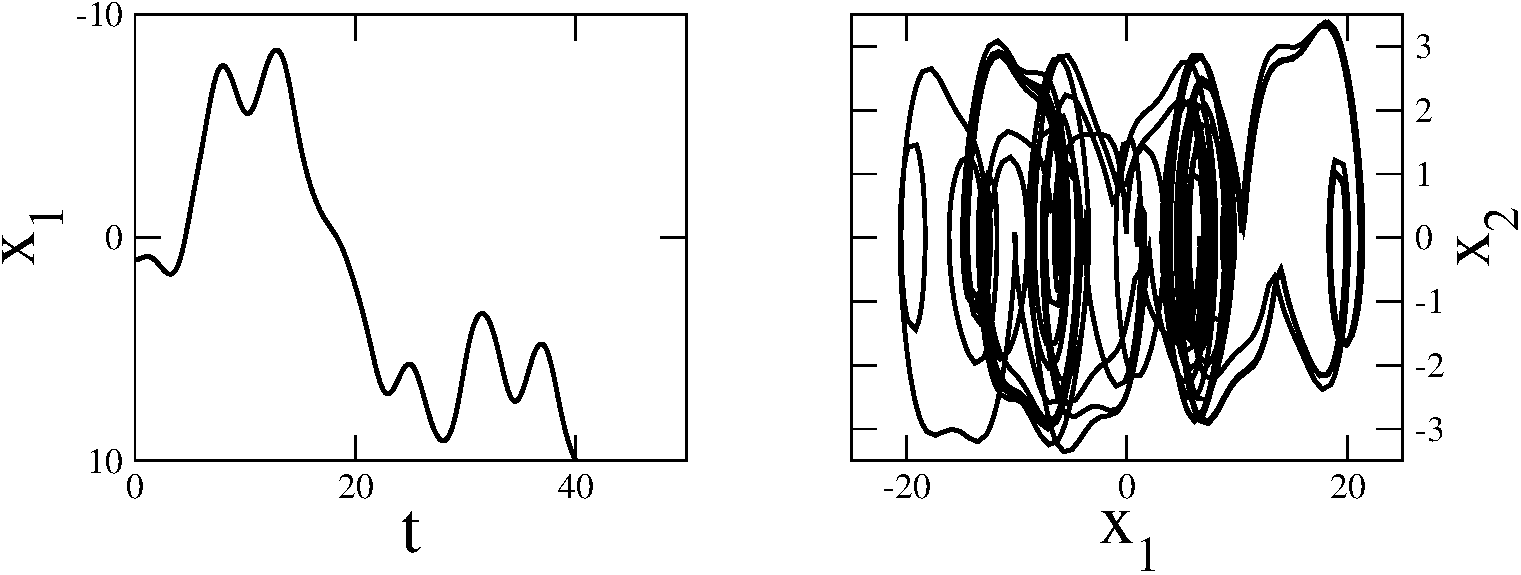
\includegraphics[draft=false,width=1.0\textwidth]{damped_driven.pdf}}
\end{minipage}

\end{frame}







\rem{
\begin{frame}[fragile]

  \heading{Different Steppers}

  \vspace{2ex}

  \begin{lstlisting}
runge_kutta_fehlberg78< state_type > s;
  \end{lstlisting}

  \begin{lstlisting}
runge_kutta_dopri5< state_type > s;
  \end{lstlisting}

  \vspace{2ex}
  Symplectic steppers (for Hamiltonian systems)
  \begin{lstlisting}
symplectic_rkn_sb3a_mclachlan< state_type > s;
  \end{lstlisting}

  \vspace{2ex}
  Implicit steppers (for stiff systems)
  \begin{lstlisting}
rosenbrock4< double > s;
  \end{lstlisting}

  \vspace{2ex}
  {\bf These steppers perform one step with constant step size!}

\end{frame}
}






\begin{frame}
 
 \heading{Controlled steppers -- Step size control}

 \only<1>{
\centerline{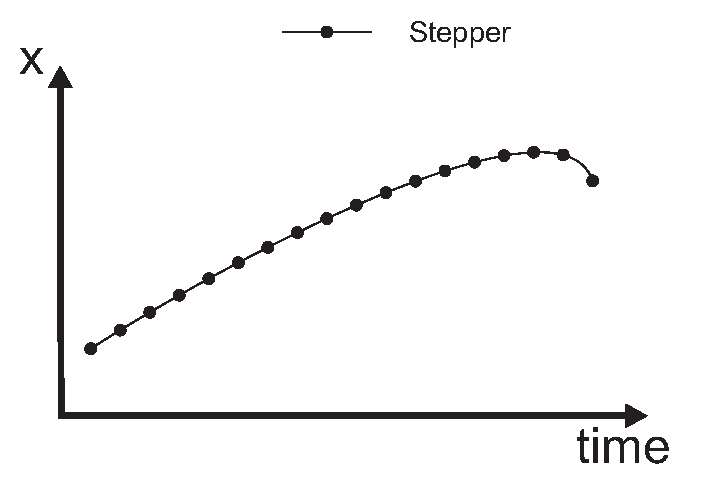
\includegraphics[draft=false,width=0.8\textwidth]{controlled_stepper1.pdf}}
 }
 \only<2>{
\centerline{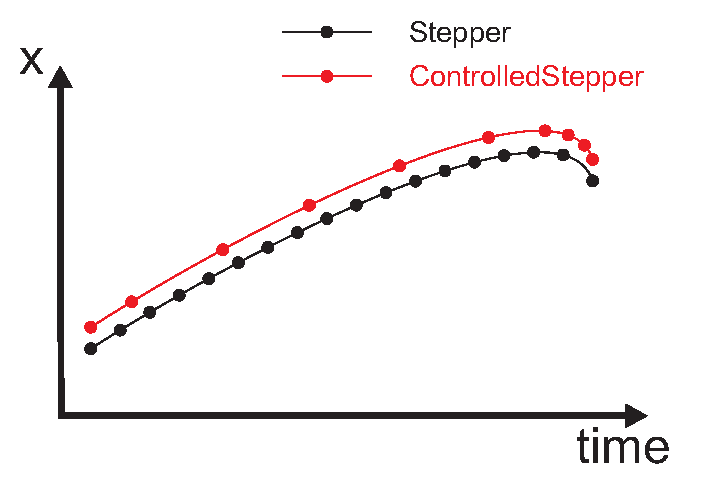
\includegraphics[draft=false,width=0.8\textwidth]{controlled_stepper2.pdf}}
 }


 
\end{frame}



\begin{frame}[fragile]
 
 \heading{Controlled steppers}
 
 \vspace{2ex}

 \begin{lstlisting}
auto s = make_controlled( 1.0e-6 , 1.0e6,
  runge_kutta_fehlberg78<state_type>() );

controlled_step_result res = 
  s.try_step(ode,x,t,dt);
 \end{lstlisting}

 Tries to perform the step and updates $x$, $t$, and $dt$!

 \vspace{4ex}


 It works because Runge-Kutta-Fehlberg has error estimation:

 \begin{lstlisting}
runge_kutta_fehlberg78<state_type> s;
s.do_step(ode,x,t,dt,xerr);
 \end{lstlisting}


\end{frame}


\begin{frame}[fragile]

\heading{Controlled steppers}

\vspace{2ex}

\begin{lstlisting}
auto s = make_controlled(1.0e-6,1.0e6,
  runge_kutta_fehlberg78<state_type>() );
while( t < t_end )
{
  controlled_step_result res;
  do
  { 
    res = s.try_step(ode,x,t,dt);
  }
  while( res != success )
}
\end{lstlisting}

\centerline{Non-trivial time-stepping logic}

\end{frame}


\begin{frame}[fragile]

  \heading{Use integrate functions!}

\vspace{2ex}


\begin{lstlisting}
integrate_adaptive(s,ode,x,t_start,t_end,dt); 
integrate_adaptive(s,ode,x,t_start,t_end,dt,observer);
\end{lstlisting}

Observer: Callable object {\tt obs(x,t)}

\vspace{4ex}
Example (using Boost.Phoenix):
\begin{lstlisting}
integrate_adaptive(s,ode,x,t_start,t_end,dt,
  cout << arg1[0] << " " << arg1[1] << "\n" );
\end{lstlisting}

\vspace{2ex}
More integrate versions:

{\tt integrate\_const}, {\tt integrate\_times}, \dots

\end{frame}



\begin{frame}[fragile]

\heading{Adaptive step size vs. constant step size}

\vspace{2ex}

\begin{lstlisting}
integrate_const(s,ode,x,t,dt,obs);
\end{lstlisting}
\begin{lstlisting}
integrate_adaptive(s,ode,x,t,dt,obs);
\end{lstlisting}

\vspace{2ex}

\centerline{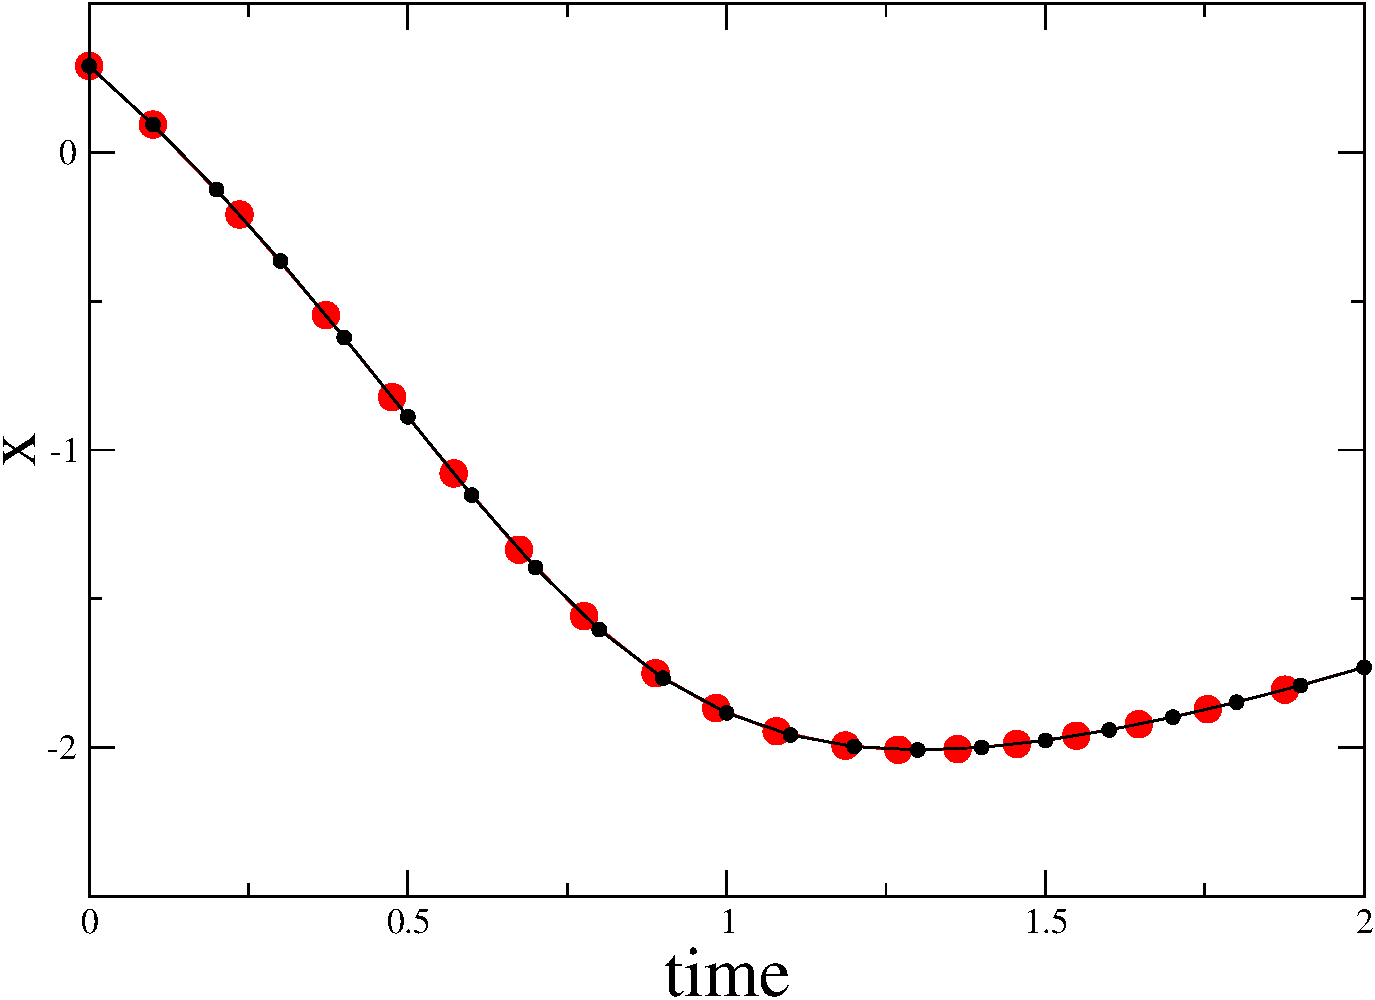
\includegraphics[draft=false,width=0.6\textwidth]{vdp_dense_output.pdf}}

\textbf{Problem:} Equidistant observation with adaptive step size integration?


\end{frame}



\begin{frame}[fragile]

\heading{Dense output stepper}

\vspace{2ex}

\begin{lstlisting}
auto s = make_dense_output( 1.0e-6 , 1.0e-6 ,
    runge_kutta_dopri5< state_type >() );
integrate_const( s , p , x , t , dt );
\end{lstlisting}

Interpolation within integration interval with the same precision as the stepper!

\vspace{2ex}

\centerline{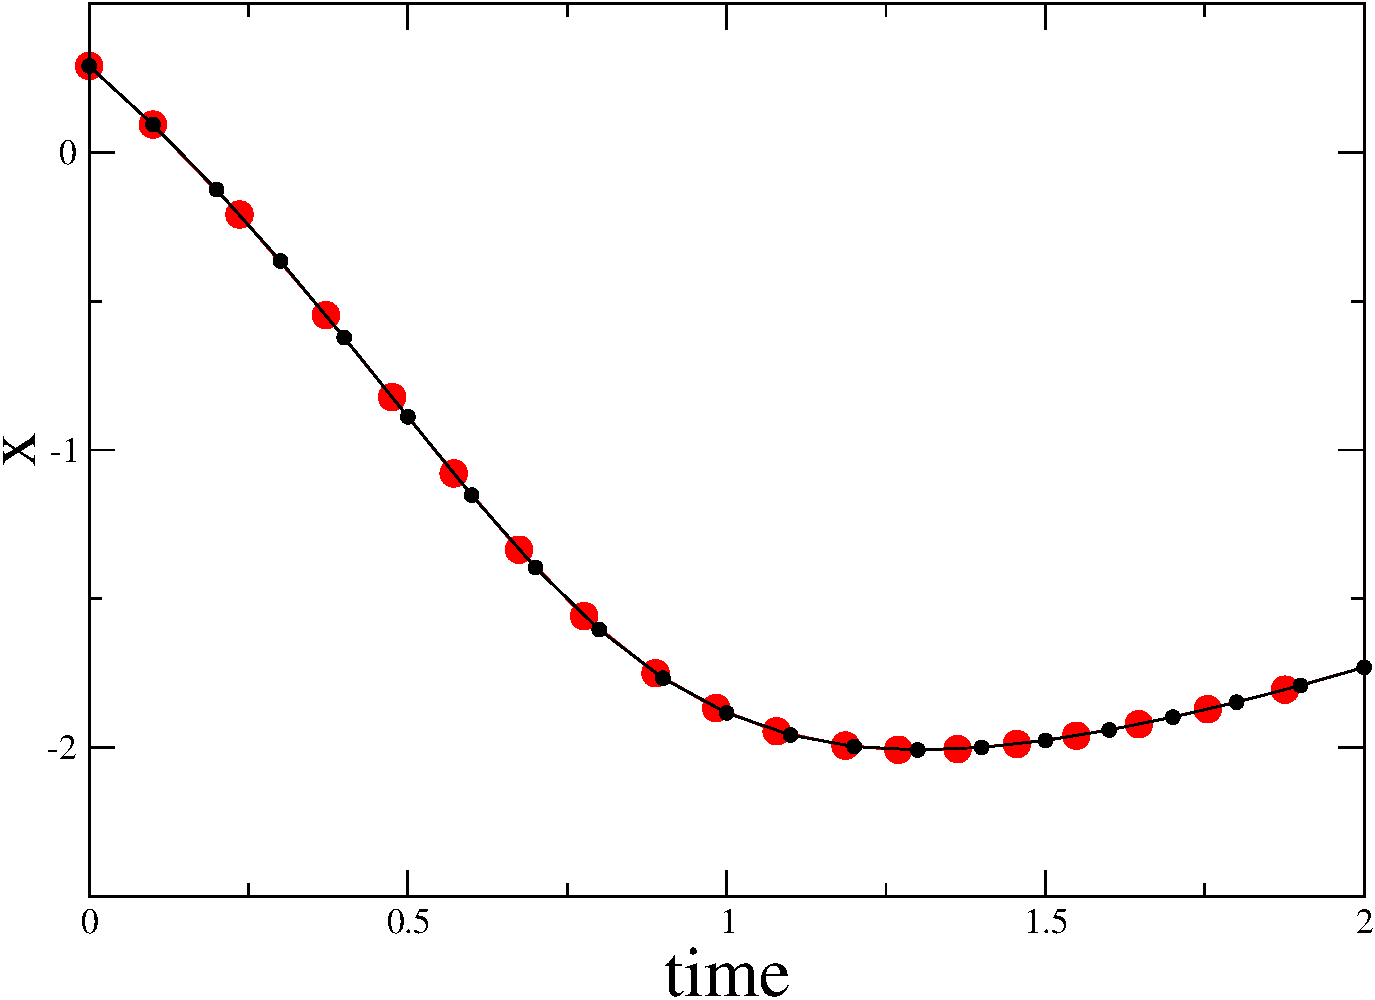
\includegraphics[draft=false,width=0.6\textwidth]{vdp_dense_output.pdf}}

\end{frame}







\begin{frame}
 \heading{More steppers}

 \vspace{2ex}

 {\bf Stepper Concepts}: Stepper, ErrorStepper, ControlledStepper, DenseOutputStepper

 \vspace{2ex}

 {\bf Stepper types}: 
 \begin{itemize}
  \item Implicit -- {\tt implicit\_euler}, {\tt rosenbrock4}
  \item Symplectic -- {\tt symplectic\_rkn\_sb3a\_mclachlan}
  \item Predictor-Corrector -- {\tt adams\_bashforth\_moulton}
  \item Extrapolation -- {\tt bulirsch\_stoer}
  \item Multistep methods -- {\tt adams\_bashforth\_moulton}
 \end{itemize}

 \vspace{2ex}
 Some of them have step-size control and dense-output!

 \vspace{2ex}

 For details see the odeint documentation!

\end{frame}





\begin{frame}
 
 \heading{Small summary}

 \vspace{2ex}
 \begin{itemize}
  \item Very easy example -- nonlinear driven pendulum
  \item Basic features of \odeint
  \item Different steppers -- steppers, error steppers, controlled steppers, dense output steppers
  \item Integrate functions
 \end{itemize}

 \vspace{2ex}

 \pause
 \centerline{\bf Now, let's look at some advanced features!}

\end{frame}



\begin{frame}
 
\heading{Large systems}

\vspace{2ex}

\begin{minipage}{0.48\textwidth} \begin{center}
  Lattice systems

  \vspace{3ex}

  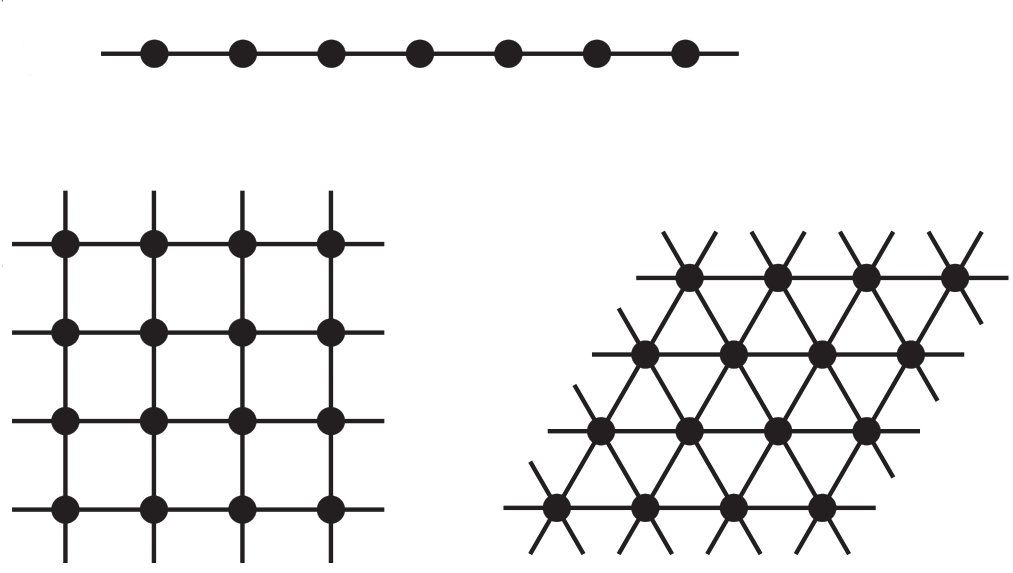
\includegraphics[draft=false,width=0.8\textwidth]{lattices.jpg}
\end{center} \end{minipage}
\pause
\begin{minipage}{0.48\textwidth} \begin{center}
  Discretiztations of PDEs

  \vspace{0.5ex}
  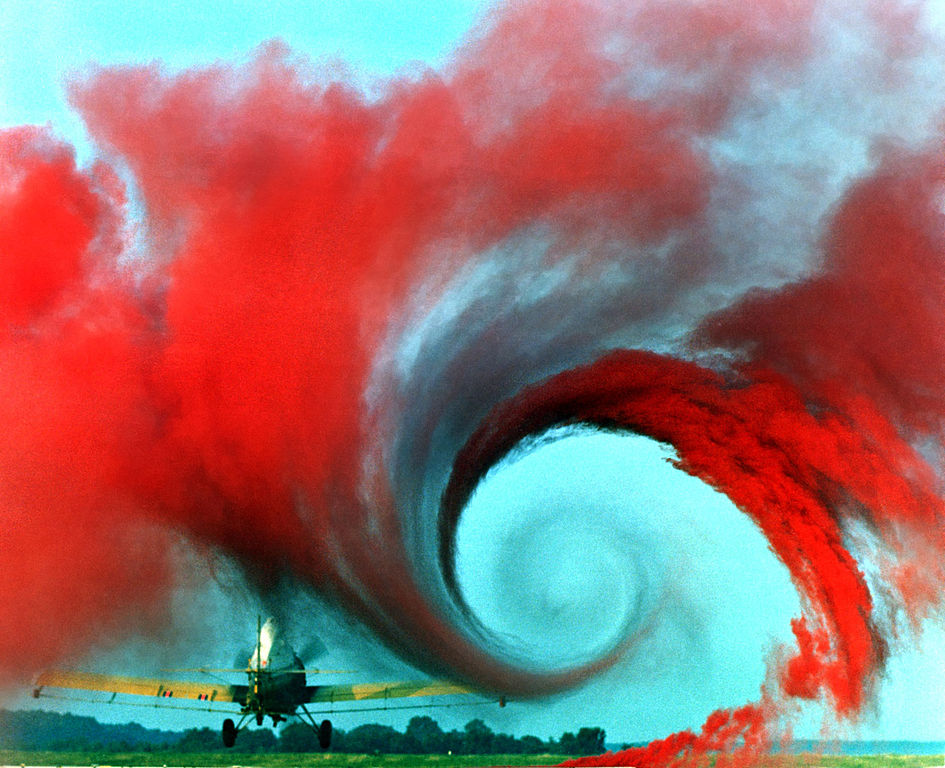
\includegraphics[draft=false,width=0.7\textwidth]{turbulence.jpg}
\end{center} \end{minipage}

\pause
\vspace{2ex}

\begin{minipage}{0.48\textwidth}\begin{center}
  ODEs on graphs

  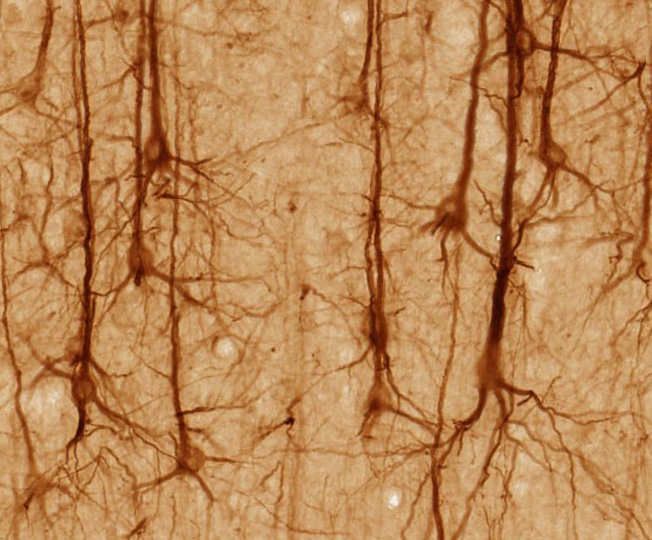
\includegraphics[draft=false,width=0.7\textwidth]{neuron.jpg}
 \end{center}\end{minipage}\pause
\begin{minipage}{0.48\textwidth}\begin{center}
  Parameter studies
 
  \vspace{0.5ex}
  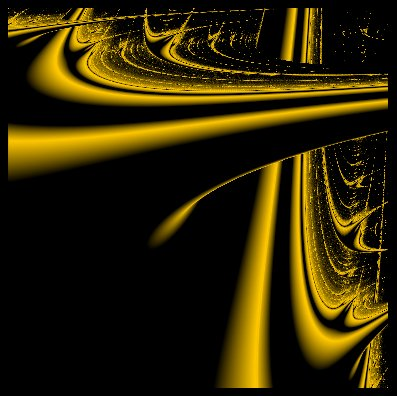
\includegraphics[draft=false,width=0.59\textwidth]{lyap.jpg}
 \end{center} \end{minipage}

 \vspace{2ex}
 \centerline{\bf High-Performance-Computing}


\end{frame}







\rem{
\begin{frame}[fragile]
 \heading{Coupled phase oscillators}

 \vspace{2ex}

 \begin{columns}[T]
  \begin{column}{0.35\textwidth}
   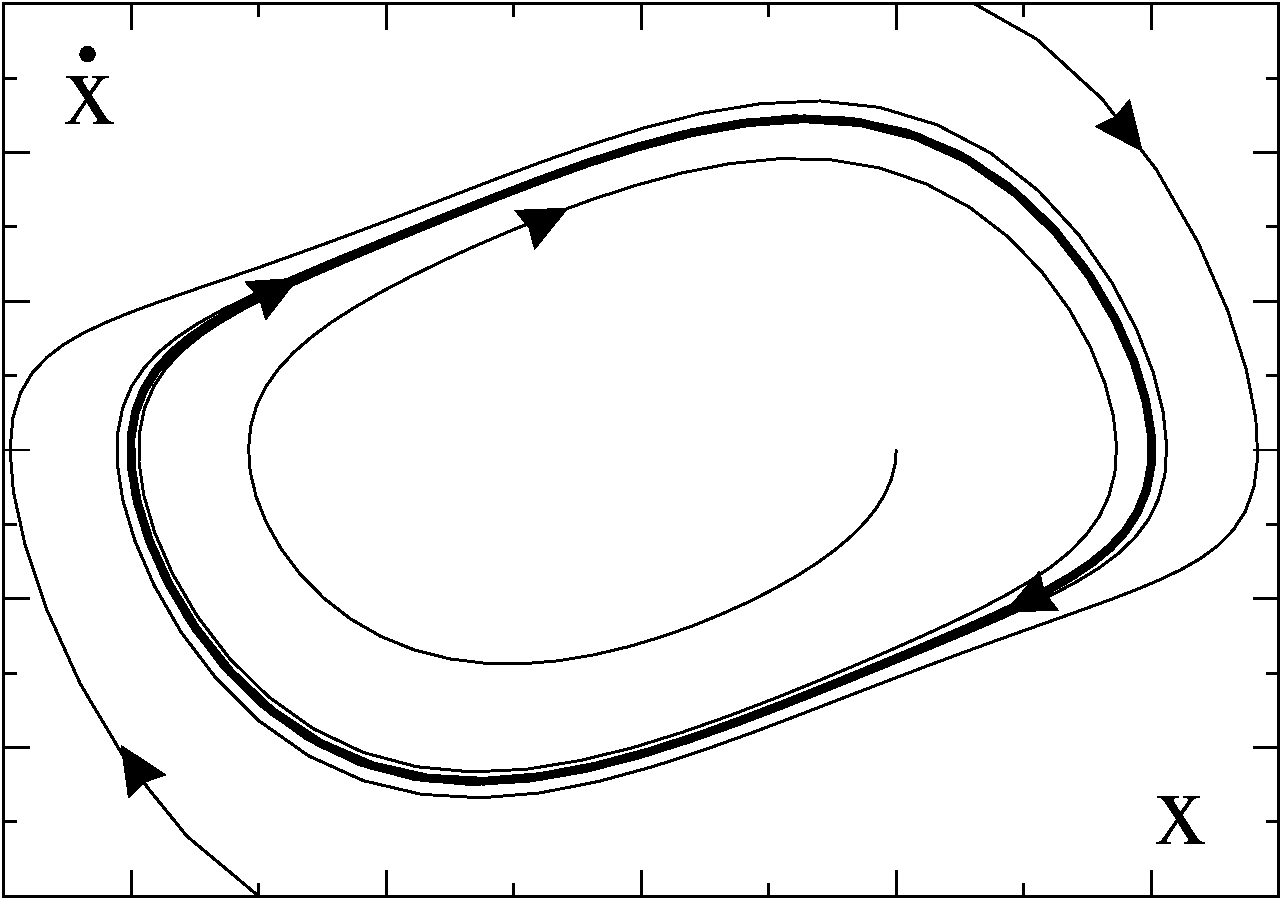
\includegraphics[draft=false,width=1.0\textwidth]{vdp.pdf}  
  \end{column}
  \begin{column}{0.63\textwidth}
 Any oscillator can be described by one variable -- its phase!

 \vspace{2ex}

 Trivial dynamic: $\dot{\varphi}=\omega$

  \end{column}
 \end{columns}

 \pause


 \vspace{2ex}

 Interesting behaviour occurs if oscillators are coupled.

 \begin{itemize}
  \item Synchronization, oscillation death, phase chaos, pattern formation, \dots
 \end{itemize}

 Applications: Neurosciences, Heart dynamics, social systems

 \vspace{2ex}

 Any weakly coupled oscillator system

 \vspace{1ex}

 \centerline{$\dot{\varphi}_k = \omega_k + q( \varphi_{k+1} , \varphi_k ) + q( \varphi_k , \varphi_{k-1} )$}

   
 
\end{frame}
}



\begin{frame}[fragile]
 
 \heading{Phase compacton lattice}

 \vspace{2ex}

 $$\dot{\varphi}_k = \cos \varphi_{k+1} - \cos \varphi_{k-1}$$

 \vspace{2ex}

 State space contains $N$ variables

 \begin{lstlisting}
typedef std::vector<double> state_type;
 \end{lstlisting}

 \vspace{2ex}

 \centerline{Simulation}

\end{frame}

\begin{frame}[fragile]

 \heading{Phase compacton lattice -- Space-time plots}

 \vspace{2ex}

\centerline{\begin{sideways}\hspace{0ex}spatial index\end{sideways} 
\includegraphics[draft=false,width=0.9\textwidth]{transition_chaos_1.jpg}}

\centerline{time}


\vspace{4ex}
\centerline{\begin{sideways}\hspace{0ex}spatial index\end{sideways} 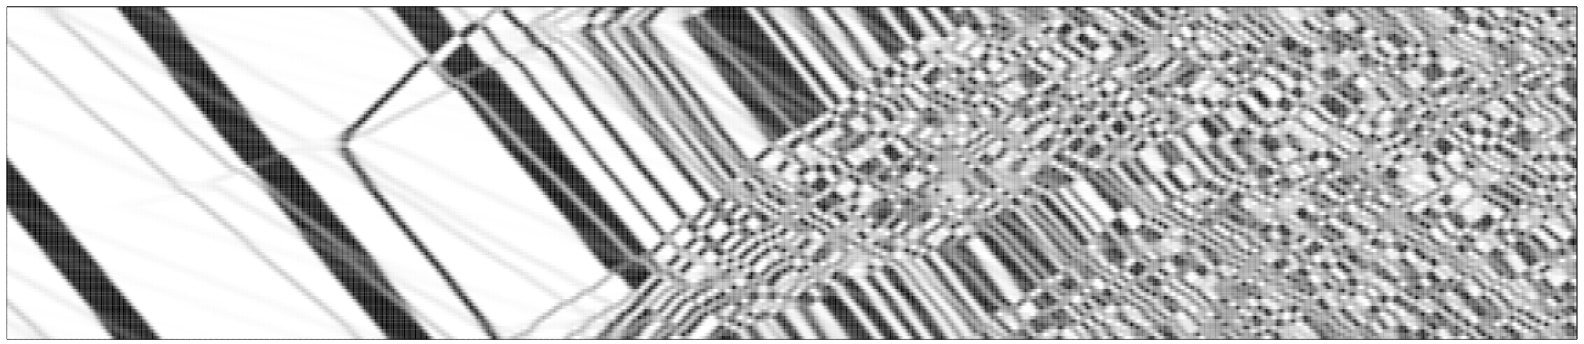
\includegraphics[draft=false,width=0.9\textwidth]{transition_chaos_2.jpg}}

\centerline{time}
 
\end{frame}








\rem{
\begin{frame}[fragile]

 \heading{Ensemble of phase oscillators -- SKIP}

 \vspace{2ex}

$$\dot{\varphi}_k = \omega_k + \sum\limits_l \sin( \varphi_l - \varphi_k )$$

{\bf Synchronization} -- all oscillator oscillates with the same frequency

 \vspace{2ex}

Synchronized state $\varphi_k = \omega_S t + \varphi_{0,k} $

\end{frame}





\begin{frame}[fragile]

\heading{Ensemble of phase oscillators -- SKIP}

\begin{lstlisting}
typedef std::vector<double> state_type;

struct ensemble
{
    state_type m_omega,m_eps;

    ensemble(size_t n,double eps)
    : m_omega(n,0.0),m_eps(eps)
    {
        create_frequencies();
    }

    void create_frequencies() { ... }

    void operator()(const state_type &x,state_type &dxdt,double t) const
    {
         ...
    }
};
\end{lstlisting}

The ODE has now many parameters, use boost::ref

Vielleicht koennen diese beiden Folien weg

\end{frame}
}


\begin{frame}[fragile]

\heading{Solving ODEs with CUDA using Thrust}

\vspace{4ex}
\begin{quotation}
``Thrust is a parallel algorithms library which resembles the C++ Standard Template Library (STL). Thrust's high-level interface greatly enhances developer productivity while enabling performance portability between GPUs and multicore CPUs. Interoperability with established technologies (such as CUDA, TBB and OpenMP) facilitates integration with existing software. Develop high-performance applications rapidly with Thrust!''
\end{quotation}

\vspace{2ex}

\centerline{
\includegraphics[draft=false,width=0.3\textwidth]{thrust_logo.png}}
 

\end{frame}


\begin{frame}[fragile]
 
\heading{Solving ODEs with CUDA using thrust}

\vspace{2ex}
Applications and use cases for GPUs:

\begin{itemize}
 \item Large systems, discretizations of PDEs, lattice systems, granular systems, etc.
 \item Parameter studies, solve many ODEs in parallel with different parameters
 \item Initial value studies, solve the same ODE with many different initial conditions in parallel
\end{itemize}


\end{frame}



\begin{frame}[fragile]
 
\heading{Lorenz system -- Deterministic chaos}

 $$
  \dot{x} = \sigma ( y - x ) \quad \quad \dot{y} = R x - y - x z \quad \quad \dot{z} = -b z + x y
 $$

Standard parameters $\sigma=10$, $R=28$, $b=8/3$

\vspace{2ex}
Perturbations grow exponentially fast -- Butterfly effect

\vspace{4ex}

\centerline{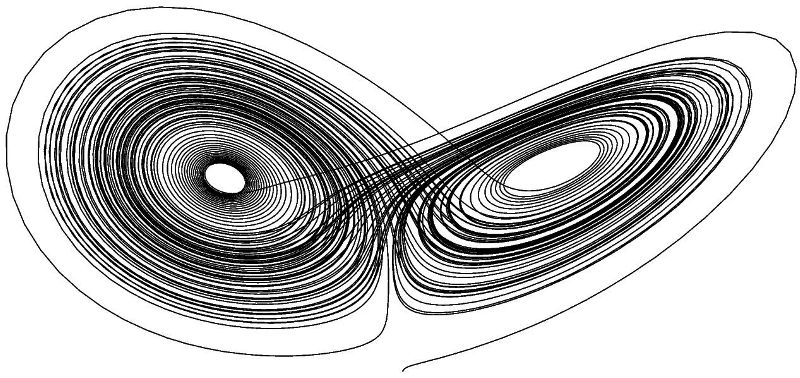
\includegraphics[draft=false,width=0.8\textwidth]{lorenz.jpg}}



\end{frame}


\begin{frame}[fragile]
 
  \heading{Lorenz system -- Parameter study}


 $$
  \dot{x} = \sigma ( y - x ) \quad \quad \dot{y} = R x - y - x z \quad \quad \dot{z} = -b z + x y
 $$


Does one observe chaos over the whole parameter range?

\vspace{2ex}

Lyapunov exponents:
\begin{itemize}
 \item Measure of chaos
 \item Growth rate of perturbations
\end{itemize}

\vspace{2ex}
Vary $R$ from $0$ to $50$ and calculate the Lyapunov exponents!

\vspace{2ex}
\centerline{\bf Use CUDA and Thrust!}

\end{frame}


\begin{frame}[fragile]

 \heading{Intermezzo: Algebras and operations}

 \vspace{2ex}

Euler method

$$\text{for all i :}  \quad \quad x_i(t+\Delta t) = x_i(t) + \Delta t \cdot f_i(x)$$

\vspace{2ex}

\begin{lstlisting}
typedef euler< state_type ,
   value_type , deriv_type , time_type,
   algebra , operations , resizer > stepper; 
\end{lstlisting}


\begin{itemize}
\item Algebras perform the iteration over $i$.
\item Operations perform the elementary addition.
\end{itemize}


\end{frame}

\begin{frame}[fragile]

 \heading{Intermezzo: Algebras and operations}

\begin{lstlisting}
typedef euler< state_type ,
   value_type , deriv_type , time_type,
   algebra , operations , resizer > stepper; 
\end{lstlisting}

Default template parameters:

\begin{itemize}
 \item {\tt range\_algebra} -- Boost.Ranges
 \item {\tt default\_operations}
\end{itemize}

\vspace{2ex}
For Thrust:

\begin{itemize}
 \item {\tt thrust\_algebra}
 \item {\tt thrust\_operations}
\end{itemize}

 
\end{frame}



\begin{frame}[fragile]

 \heading{Calculate an ensemble of Lorenz systems}

 \begin{lstlisting}[basicstyle=\scriptsize\ttfamily]
typedef thrust::device_vector<double> state_type;
typedef runge_kutta4<state_type,double,state_type,double,
   thrust_algebra,thrust_operations> stepper; 

state_type x( 3*N );
// initialize x
integrate_const( stepper() , lorenz_ensemble() ,
   x , 0.0 , 1000.0 , dt );
 \end{lstlisting}

\vspace{2ex}

\centerline{Memory layout:}

\vspace{1ex}

\centerline{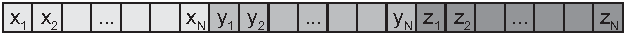
\includegraphics[draft=false,width=0.9\textwidth]{memory_layout.pdf}}

\vspace{6ex}

\centerline{Everything seems easy!}
\vspace{2ex}
\centerline{{\bf But} how does {\tt lorenz\_ensemble} look like?}
 

\end{frame}




\begin{frame}[fragile]

 \heading{Ensemble of Lorenz systems}

 \begin{lstlisting}[basicstyle=\scriptsize\ttfamily]
struct lorenz_ensemble {
  size_t N;
  state_type beta;

  template< class State , class Deriv >
  void operator()(
    const State &x , Deriv &dxdt , value_type t ) const {
  
    thrust::for_each(
      thrust::make_zip_iterator( thrust::make_tuple(
        x.begin() , x.begin()+N , x.begin()+2*N ,
        beta.begin() ,
        dxdt.begin(), dxdt.begin()+N, dxdt.begin()+2*N
      ) ) ,
      thrust::make_zip_iterator( thrust::make_tuple(
        x.begin()+N , x.begin()+2*N , x.begin()+3*N ,
        beta.end() ,
        dxdt.begin()+N,dxdt.begin()+2*N,dxdt.begin()+3*N
      ) ) ,
      lorenz_functor() );
  }

  // ...
};
 \end{lstlisting}


\end{frame}


\begin{frame}[fragile]

 \heading{Ensemble of Lorenz systems}

 \begin{lstlisting}[basicstyle=\scriptsize\ttfamily]
struct lorenz_ensemble
{
  // ...

  struct lorenz_functor
  {
    template< class T > __host__ __device__
    void operator()( T t ) const
    {
      value_type R = thrust::get< 3 >( t );
      value_type x = thrust::get< 0 >( t );
      value_type y = thrust::get< 1 >( t );
      value_type z = thrust::get< 2 >( t );
      thrust::get< 4 >( t ) = sigma * ( y - x );
      thrust::get< 5 >( t ) = R * x - y - x * z;
      thrust::get< 6 >( t ) = -b * z + x * y ;
    }
  };
};
 \end{lstlisting}


\end{frame}




\begin{frame}[fragile]

 \heading{Lorenz system parameter study -- Results}

 \vspace{4ex}

\centerline{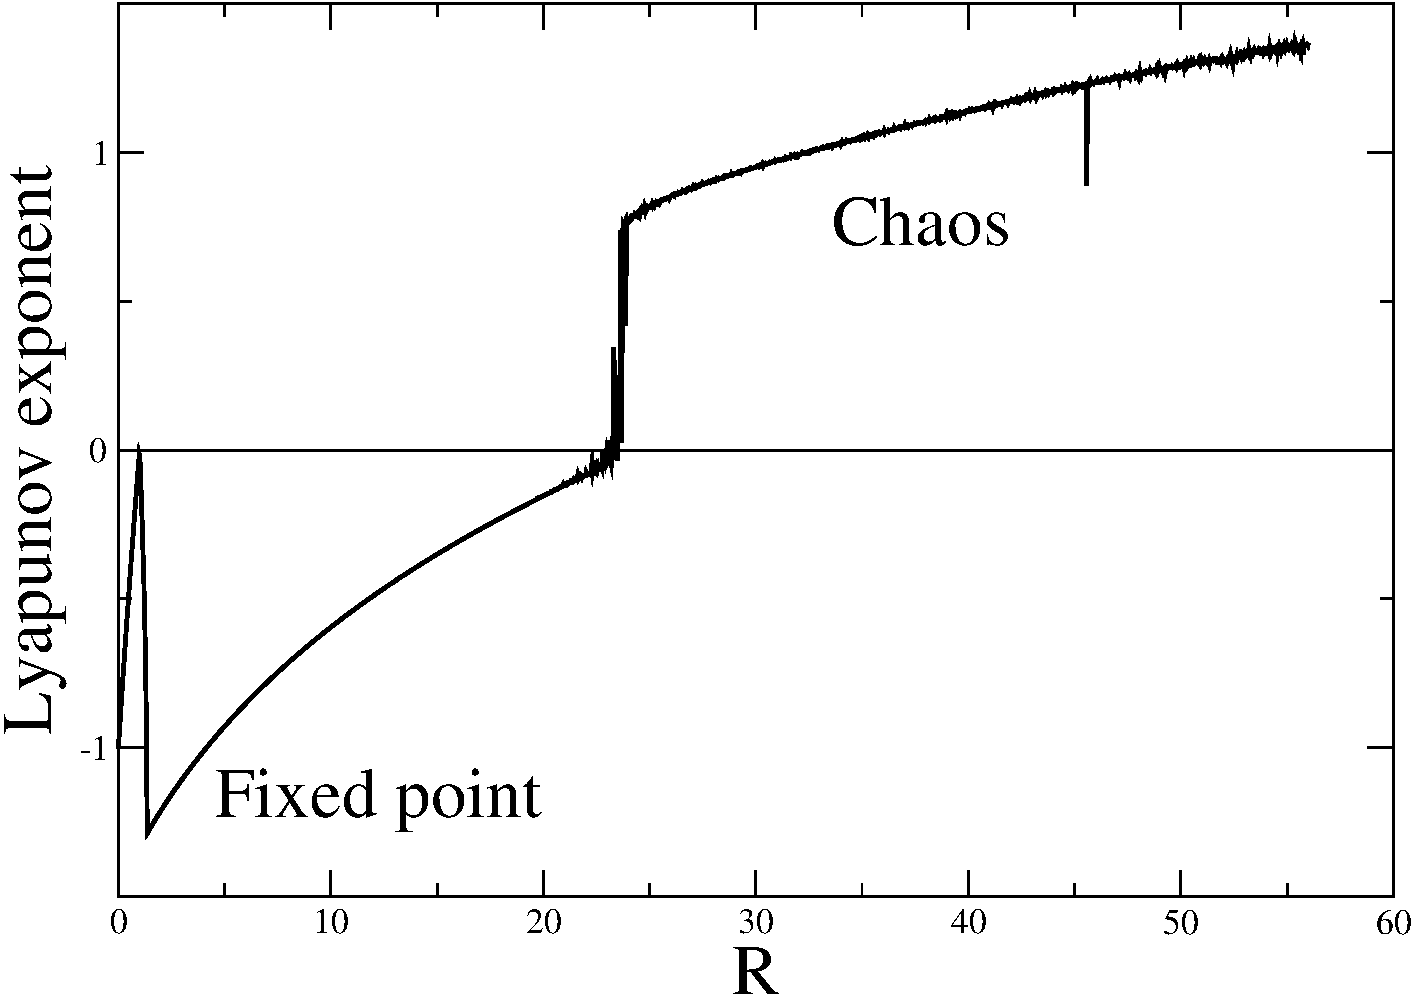
\includegraphics[draft=false,width=0.8\textwidth]{lyap_lorenz.pdf}}

\end{frame}







\begin{frame}
 \heading{Advanced features - continued}

\end{frame}


\begin{frame}[fragile]
 \heading{Reference wrapper {\tt std::ref}, {\tt boost::ref}}

\vspace{2ex}

 The ODE and the observers are always passed by value

 \begin{lstlisting}
integrate_const{s,ode,x,0.0,1.0,dt,obs);
s.do_step(ode,x,t,dt);
 \end{lstlisting}

\pause

\vspace{2ex}
Use {\tt std::ref} or {\tt boost::ref} to pass by reference
 \begin{lstlisting}
integrate_const{s,std::ref(ode),x,0.0,1.0,dt,
  std::ref(obs));
 \end{lstlisting}

\end{frame}



\begin{frame}[fragile]
 \heading{Using Boost.Range}

 \vspace{2ex}
 Use Boost.Range to integrate separate parts of the overall state

 \vspace{2ex}
 Example: Lyapunov exponents for the Lorenz system

 \vspace{2ex}

 \centerline{\bf Complete ODE = Lorenz system + Perturbation}


 \begin{itemize}
  \item Calculate transients by solving only the Lorenz system (initialize $x,y,z$)
  \item Solve whole system (state + perturbations)
 \end{itemize}

\vspace{2ex}

 \begin{lstlisting}
std::vector<double> x(6,0.0);
integrate(s,lorenz,
  make_pair(x.begin(),x.begin()+3),
  0.0,10.0,dt);
integrate(s,lorenz_pert,x,10.0,1000.0,dt);
 \end{lstlisting}



\end{frame}



\begin{frame}[fragile]
 \heading{ODEs with complex numbers}

 \vspace{2ex}

 Discrete Nonlinear Schr\"odinger equation
$$
  \ii \dot{\Psi}_k = \varepsilon_k \Psi_k + V( \Psi_{k+1}+\Psi_{k-1}) - \gamma |\Psi_k|^2 \Psi_k
  \quad \quad \text{,} \quad \Psi_k \in \mathbb{C}
$$
 

 \begin{lstlisting}[basicstyle=\scriptsize\ttfamily]
typedef std::vector<std::complex<double> > state_type;

struct dnls
{
  std::vector<double> eps;
  void operator()(const state_type &x, state_type &dxdt,
    double t) const
  {
    // ...
  }
};

runge_kutta_fehlberg78< state_type > stepper;
 \end{lstlisting}

\end{frame}

\begin{frame}[fragile]
 \heading{Matrices as state types}

 \vspace{1ex}
 \begin{columns}[T]
  \begin{column}{0.35\textwidth}
   \centerline{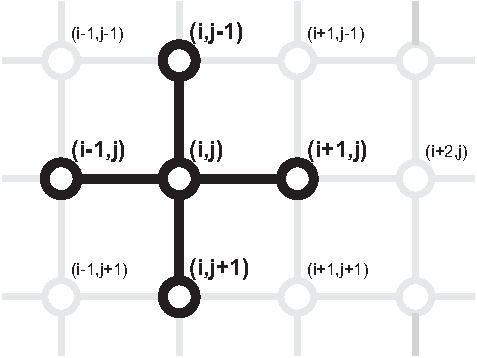
\includegraphics[draft=false,width=0.9\textwidth]{2dlattice.pdf}}
  \end{column}
  \begin{column}{0.58\textwidth}
Example: 

\vspace{1ex}
Two-dimensional phase lattice
\begin{align*}
\dot{\varphi}_{i,j} = &
  q(\varphi_{i+1,j},\varphi_{i,j}) 
 + q(\varphi_{i-1,j},\varphi_{i,j}) \\
 + & q(\varphi_{i,j+1},\varphi_{i,j}) 
 + q(\varphi_{i,j-1},\varphi_{i,j})
 \end{align*}
  \end{column}
 \end{columns}

\vspace{1ex}

\begin{lstlisting}[basicstyle=\scriptsize\ttfamily]
typedef ublas::matrix<double> state_type1;
typedef mtl::dense2D<double> state_type2;

runge_kutta_fehlberg78< state_type1 , double ,
  state_type1 , double , vector_space_algebra > stepper1;
\end{lstlisting}

\pause
\vspace{1ex}


\centerline{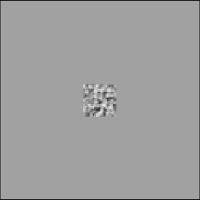
\includegraphics[draft=false,width=0.27\textwidth]{phase_lattice_2d_0000.jpg} \hspace{2ex}
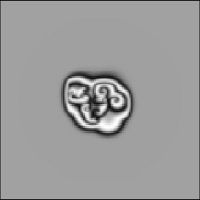
\includegraphics[draft=false,width=0.27\textwidth]{phase_lattice_2d_0100.jpg} \hspace{2ex}
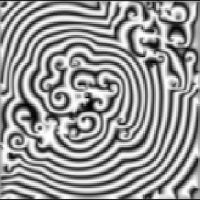
\includegraphics[draft=false,width=0.27\textwidth]{phase_lattice_2d_1000.jpg}}
\end{frame}

\begin{frame}[fragile]
 \heading{Compile-time sequences and Boost.Units}

 $$
 \left( \begin{array}{c} \dot{x} \\ \dot{v} \end{array} \right) 
= \left( \begin{array}{l} v \\ f(x,v) \end{array} \right)
$$
 \begin{itemize}
  \item $x$ -- length, dimension $m$
  \item $v$ -- velocity, dimension $m s^{-1}$
  \item $a$ -- acceleration, dimension $m s^{-2}$
 \end{itemize}

 \begin{lstlisting}[basicstyle=\tiny\ttfamily]
typedef units::quantity< si::time , double > time_type;
typedef units::quantity< si::length , double > length_type;
typedef units::quantity< si::velocity , double > velocity_type;
typedef units::quantity< si::acceleration , double > acceleration_type;

typedef fusion::vector< length_type , velocity_type > state_type;
typedef fusion::vector< velocity_type , acceleration_type > deriv_type;

typedef runge_kutta_dopri5< state_type , double , deriv_type , time_type , fusion_algebra > stepper_type;
 \end{lstlisting}

 

\end{frame}


\begin{frame}[fragile]
 \heading{What else}


\vspace{2ex}

\begin{minipage}[c]{0.35\textwidth}
\begin{itemize}\item ODEs on graphs\end{itemize}
\end{minipage} \hspace{1ex}
\begin{minipage}[c]{0.6\textwidth}
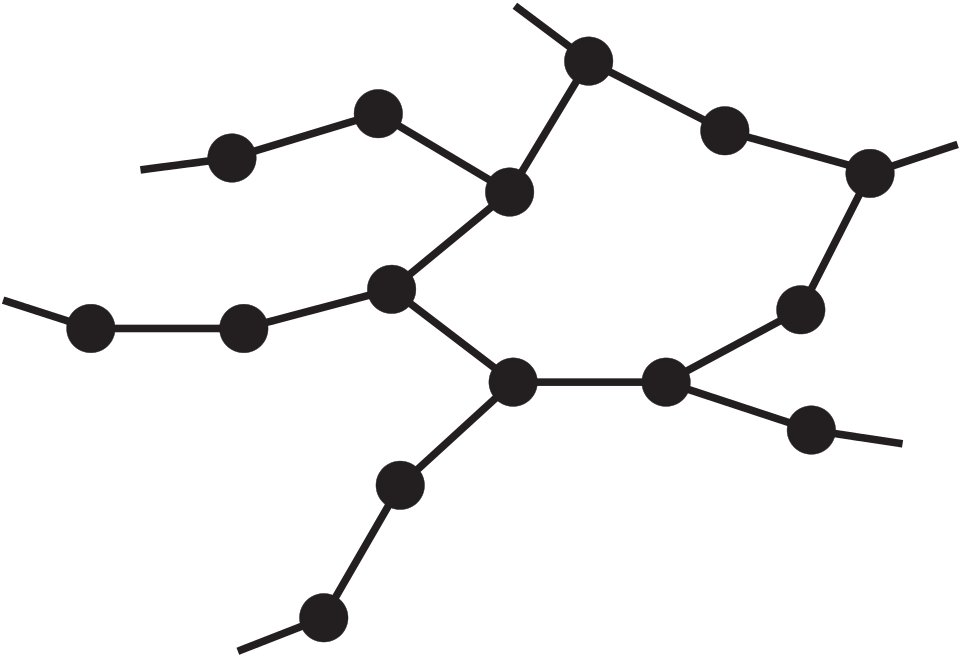
\includegraphics[draft=false,width=0.5\textwidth]{graph.jpg}
\end{minipage}
\pause

\vspace{2ex}
\begin{minipage}[c]{0.35\textwidth}
\begin{itemize}\item Automatic memory management\end{itemize}
\end{minipage} \hspace{1ex}
\begin{minipage}[c]{0.6\textwidth}
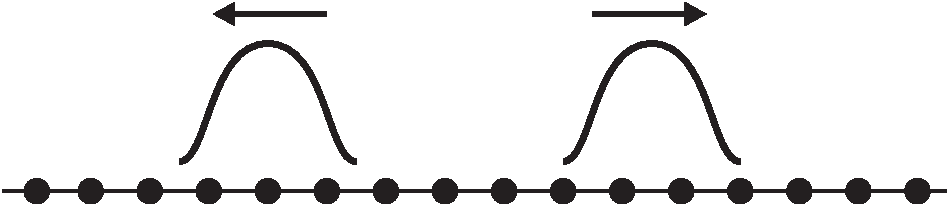
\includegraphics[draft=false,width=0.9\textwidth]{self_expanding_lattice.pdf}

\vspace{0.5ex}
{\scriptsize Enlarge the lattice when waves hit the boundaries}
\end{minipage}
\pause

\vspace{2ex}
\begin{itemize}\item Arbitrary precision types, GMPXX\end{itemize}



\end{frame}
